\documentclass{standalone}
\usepackage{graphicx}	
\usepackage{amssymb, amsmath}
\usepackage{color}

\usepackage{tikz}
\usetikzlibrary{intersections, backgrounds, math}
\usepackage{pgfmath}

\definecolor{light}{RGB}{220, 188, 188}
\definecolor{mid}{RGB}{185, 124, 124}
\definecolor{dark}{RGB}{143, 39, 39}
\definecolor{highlight}{RGB}{180, 31, 180}
\definecolor{gray10}{gray}{0.1}
\definecolor{gray20}{gray}{0.2}
\definecolor{gray30}{gray}{0.3}
\definecolor{gray40}{gray}{0.4}
\definecolor{gray60}{gray}{0.6}
\definecolor{gray70}{gray}{0.7}
\definecolor{gray80}{gray}{0.8}
\definecolor{gray90}{gray}{0.9}
\definecolor{gray95}{gray}{0.95}

\tikzmath{
  function normal(\x) {
    return exp(-0.5 * \x * \x);
  };
}

\begin{document}

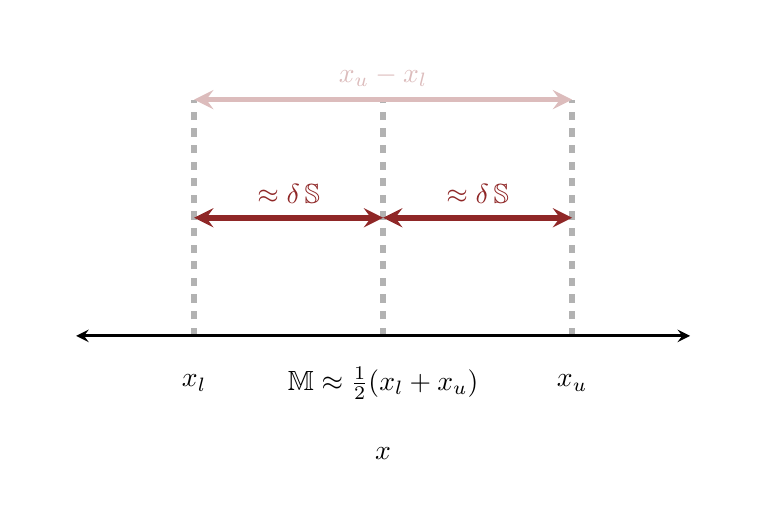
\begin{tikzpicture}[scale=0.3, thick]
  \draw[white] (-15, -15) rectangle (15, 5);

  \draw[dashed, line width=2, gray70] (-8, -8) -- +(0, 10);
  \draw[dashed, line width=2, gray70] (0, -8) -- +(0, 10);
  \draw[dashed, line width=2, gray70] (+8, -8) -- +(0, 10);
  
  \draw[<->, >=stealth, line width=2, light] (-8, 2) -- +(16, 0);
  \node[light] at (0, 3) { $x_{u} - x_{l}$ };
  
  \draw[<->, >=stealth, line width=2, dark] (-8, -3) -- +(8, 0);
  \draw[<->, >=stealth, line width=2, dark] (0, -3) -- +(8, 0);
  
  \node[dark] at (-4, -2) { $\approx \delta \, \mathbb{S}$ };
  \node[dark] at (+4, -2) { $\approx \delta \, \mathbb{S}$ };
  
  \draw [<->, >=stealth, line width=1] (-13, -8) -- +(26, 0);
  \node[] at (-8, -10) { $x_{l}$ };
  \node[] at (0, -10) { $\mathbb{M} \approx \frac{1}{2} ( x_{l} + x_{u} )$ };
  \node[] at (+8, -10) { $x_{u}$ };
  \node[] at (0, -13) { $x$ };
\end{tikzpicture}

\end{document}  